\documentclass[11pt, oneside]{article}   	% use "amsart" instead of "article" for AMSLaTeX format
\usepackage{geometry}                		% See geometry.pdf to learn the layout options. There are lots.
\geometry{letterpaper}                   		% ... or a4paper or a5paper or ... 
%\geometry{landscape}                		% Activate for for rotated page geometry
%\usepackage[parfill]{parskip}    		% Activate to begin paragraphs with an empty line rather than an indent
\usepackage{graphicx}				% Use pdf, png, jpg, or eps with pdflatex; use eps in DVI mode
								% TeX will automatically convert eps --> pdf in pdflatex		
\usepackage{amssymb}
\usepackage{amsmath}
\usepackage{parskip}
\usepackage{color}

\graphicspath{{/Users/telliott_admin/Dropbox/Tex/png/}}

\title{Basics of the hyperbolic functions}
%\author{The Author}
\date{}							% Activate to display a given date or no date

\begin{document}
\maketitle
%\section{}
%\subsection{}
\Large
\noindent

Recalling Euler's formula:
\[ e^{ix} = \cos x + i \sin x \]
we obtain a similar formula with $- ix$:
\[ e^{-ix} = \cos(-x) + i\ \sin(-x) = \cos x - i \ \sin x \]
Adding and subtracting
\[ e^{ix} +  e^{-ix} = 2 \cos x \]
\[ e^{ix} -  e^{-ix} = -2 \ i \sin x \]
The hyperbolic functions are defined similarly, but without i:
\[ 2 \cosh x = e^{x} +  e^{-x}  \]
\[ 2 \sinh x = e^{x} -  e^{-x} \]
\begin{center} 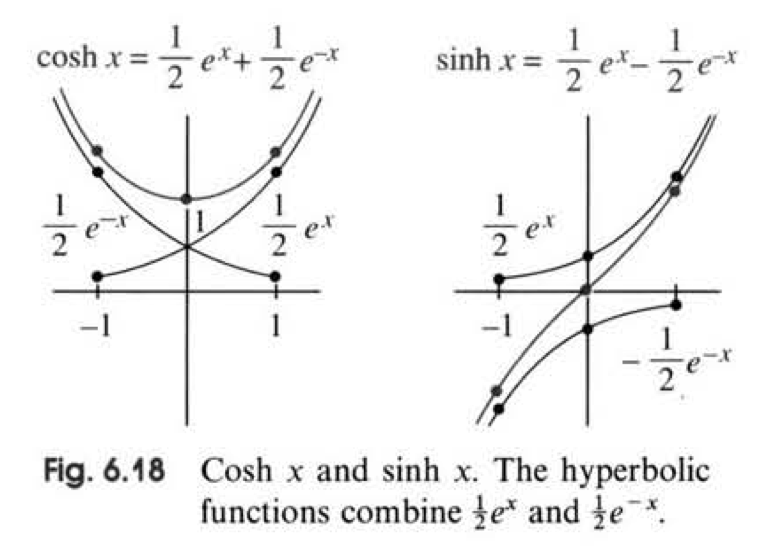
\includegraphics [scale=0.4] {cosh_and_sinh.png} \end{center}

The difference of squares has a simple value:
\[ \cosh^2 t - \sinh^2 t = 1 \]
Everything about the hyperbolic sine is reminiscent of the regular trig functions but with a sign change.

A plot of $\sinh t$ on the x-axis and $\cosh t$ on the y-axis yields a hyperbola in the same way the $y^2 - x^2 = 1$ does.

\subsection*{derivatives}
\[ \frac{d}{dx} 2 \sinh x = \frac{d}{dx} (e^x - e^{-x}) = e^x + e^{-x}  = 2 \cosh x \]
\[ \frac{d}{dx} 2 \cosh x = \frac{d}{dx} (e^x + e^{-x}) = e^x - e^{-x}  = 2 \sinh x \]

Also, note that: 
\[ 2 \sinh x + 2 \cosh x = 2 e^x \]
\[ e^x = \sinh x + \cosh x \]
Because of this, and by symmetry, we expect that the Taylor series expansions should be
\[ \sinh x = x + \frac{x^3}{3!} + \frac{x^5}{5!} + \dots \] 
\[ \cosh x = 1 + \frac{x^2}{2!} + \frac{x^4}{4!} + \dots \] 
The values of the functions at zero are
\[ \sinh 0 = 0 \]
\[ \cosh 0 = 1 \]
So, for example, the expansion for $\cosh$ is 
\[ \sinh x = \sum_{n=0}^{\infty} \frac{f^n (0)\ x^n }{n!}   \]
\[ = \frac{0 \cdot 1}{0!} + \frac{1 \cdot x}{1!} + \frac{0 \cdot x^2}{2!} + \frac{1 \cdot x^3}{3!} + \dots  \]
and so on.
\subsection*{relativity}
The hyperbolic functions come into the mathematics of relativity, where for an observer in a moving reference frame, the following equations hold:
\[ x' = \frac{x - vt}{\sqrt{1-v^2}} \]
\[ t' = \frac{t - vx}{\sqrt{1-v^2}} \]
The quantity $s^2$ is invariant where
\[ s^2 = t^2 - x^2 \]
Proof:
\[ x'^2 = \frac{x^2 - 2xvt + v^2t^2}{1-v^2} \]
\[ t'^2 = \frac{t^2 - 2xvt + v^2x^2}{1-v^2} \]
\[ t'^2 - x'^2 = \frac{t^2 - x^2 + v^2x^2 - v^2t^2}{1-v^2} \]
\[ = \frac{t^2 - x^2 + v^2(x^2 - t^2) }{1-v^2} \]
\[ = \frac{t^2 - x^2 - v^2(t^2 - x^2) }{1-v^2}  = t^2 - x^2 \]

The hyperbolic functions come in by defining a parameter $\theta$ (the "rapidity")
\[ \cosh \theta = \frac{1}{\sqrt{1-v^2}} \]
Then
\[ \sinh^2 \theta = \cosh^2 \theta - 1 = \frac{1}{1-v^2} - 1 = \frac{v^2}{1-v^2} \]
\[ \sinh \theta =  \frac{v}{\sqrt{1-v^2}} \]
So we can rewrite
\[ x' = \frac{x - vt}{\sqrt{1-v^2}} = x \cosh \theta - t \sinh \theta \]
\[ t' = \frac{t - vx}{\sqrt{1-v^2}} = t \cosh \theta - x \sinh \theta  \]
And our identity from above is
\[ t'^2 - x'^2 = (t^2 \cosh^2 \theta - 2xt \sinh \theta \cosh \theta + x^2 \sinh^2 \theta) \]
\[ \ \ \ \ \ \ \ \ \ \ - (x^2 \cosh^2 \theta - 2xt \sinh \theta \cosh \theta + t^2 \sinh^2 \theta) \]
the terms starting with $2xt$ cancel and we have
\[ t'^2 - x'^2 = (t^2 \cosh^2 \theta + x^2 \sinh^2 \theta - x^2 \cosh^2 \theta - t^2 \sinh^2 \theta) \]
\[ = t^2 (\cosh^2 \theta -  \sinh^2 \theta) - x^2  (\cosh^2 \theta -  \sinh^2 \theta) \]
\[ = t^2 - x^2  \]
\subsection*{$\tanh \theta$}
We had
\[ \sinh \theta =  \frac{v}{\sqrt{1-v^2}} \]
\[ \cosh \theta = \frac{1}{\sqrt{1-v^2}} \]
so 
\[ \tanh \theta = v \]
leading us to explore the properties of the hyperbolic tangent.  Going back to the beginning:
\[ 2 \sinh \theta = e^{\theta} -  e^{-\theta} \]
\[ 2 \cosh \theta = e^{\theta} +  e^{-\theta}  \]
\[ \tanh \theta = \frac{e^{\theta} -  e^{-\theta}}{e^{\theta} +  e^{-\theta}} \]
The derivative is (by the quotient rule):
\[ \frac{d}{d\theta} \ \tanh \theta = \frac{\cosh^2 \theta - \sinh^2 \theta}{\cosh^2 \theta}  \]
\[ =  \frac{1}{\cosh^2 \theta}  \]

Shankar has a problem involving two angles
\[ 2 \sinh ( \theta + \phi) = e^{\theta + \phi} -  e^{-\theta - \phi} \]
\[ = e^{\theta} e^{\phi} - e^{-\theta} e^{- \phi} \]

\end{document}  